\newcommand\fnote[1]{\captionsetup{font=small}\caption*{#1}}

\begin{figure*}[!t]
\begin{minipage}{.5\linewidth}
\centering
        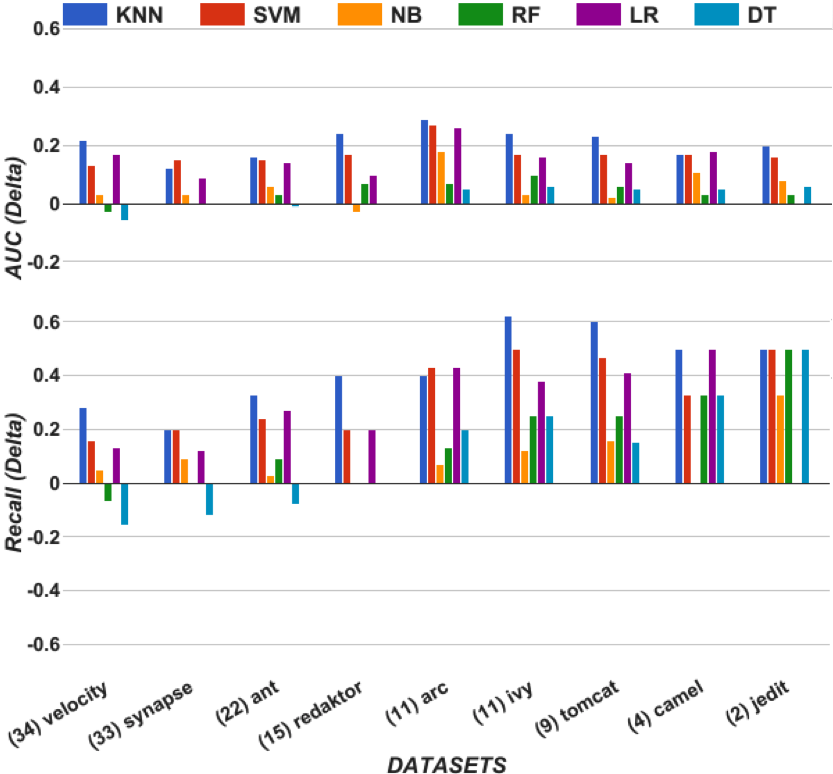
\includegraphics[width=.95\linewidth]{./fig/AUC_recall_untuned.png}
    \end{minipage}%
\begin{minipage}{.5\linewidth}
        \centering
        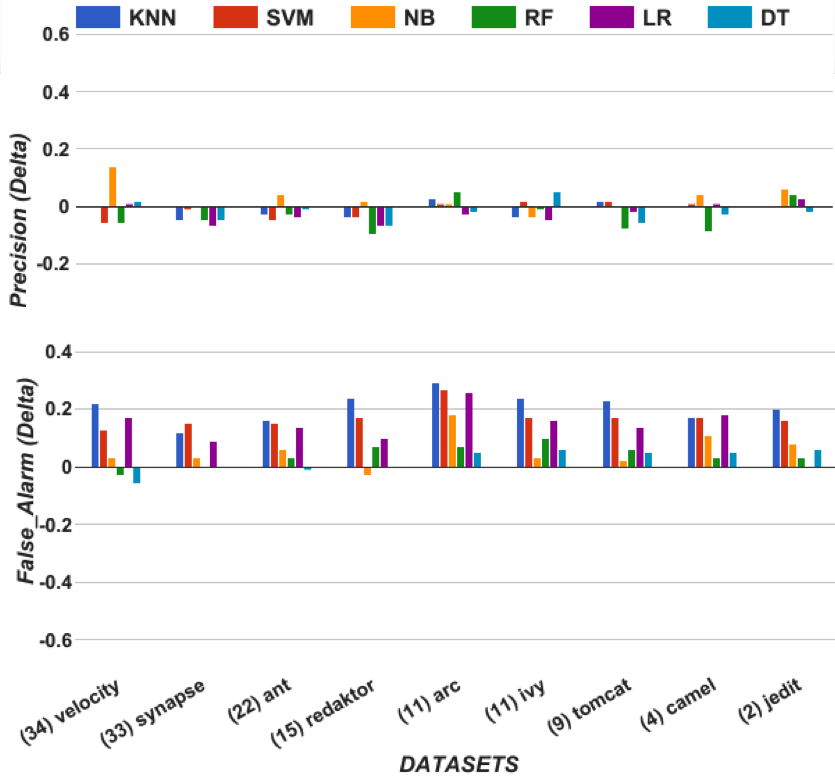
\includegraphics[width=.95\linewidth]{./fig/prec_pf_untuned.png}
    \end{minipage}%
    \caption{SMOTE1 improvement over No-SMOTE. Legends represent the classifiers mentioned in \tion{classes}}
    \vspace{-11pt}
    \fnote{For subfigures (AUC, Recall and Precision): larger y-values are {\em better}, if the y-value goes {\em negative}, then the corresponding learner trained on SMOTE1 data performs {\em worse} than learner learnt on raw data. For false alarms, the plot must be interpreted differently: larger y-values are {\em worse}, if the y-value goes {\em positive}, then the corresponding learner trained on SMOTE1 data performs {\em worse} than learner learnt on raw data. The corresponding percentage of minority class (in this case, defective class) is written beside each dataset.}
    \label{fig:untuned}
\vspace{-0.5cm}
\end{figure*}

\begin{figure*}[!htbp]
\begin{minipage}{.5\linewidth}
\centering
        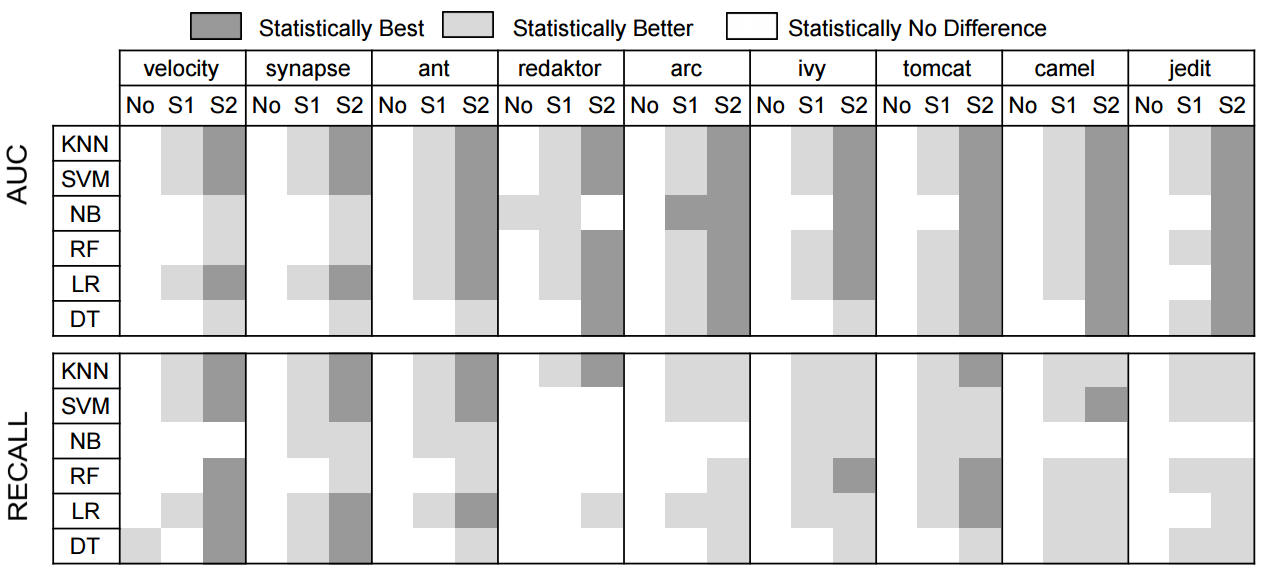
\includegraphics[width=.9\linewidth]{./fig/AUC_recall.png}
            \end{minipage}%
\begin{minipage}{.5\linewidth}
        \centering
        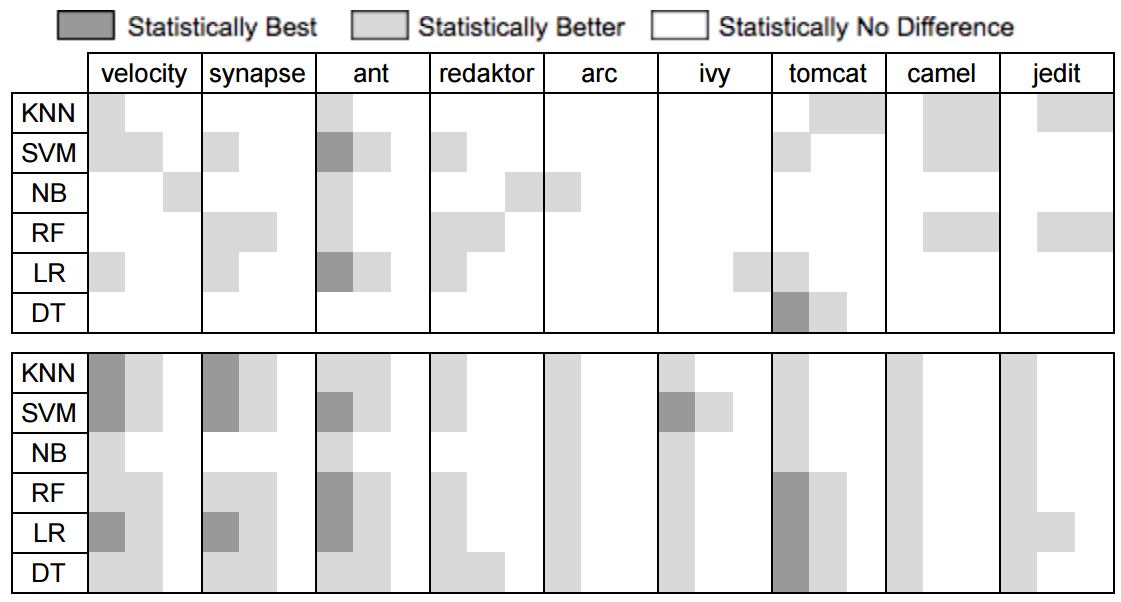
\includegraphics[width=.9\linewidth]{./fig/prec_pf.png}
    \end{minipage}%
    \caption{Scott Knott analysis of No-SMOTE, SMOTE1 and SMOTE2. The column headers are denoted as No for No-SMOTE, S1 for SMOTE1 and S2 for SMOTE2.}
    \label{fig:stats}
\vspace{-0.8cm}
\end{figure*}

\begin{figure*}[!t]
\begin{minipage}{.5\linewidth}
\centering
        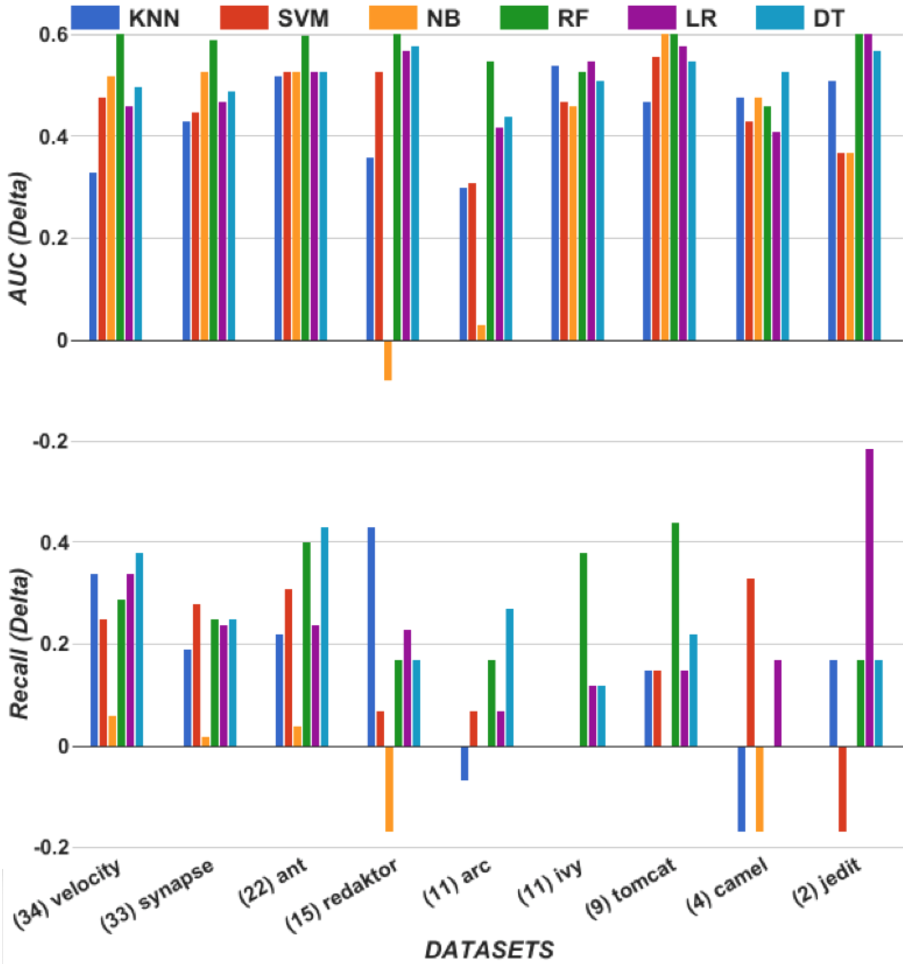
\includegraphics[width=.95\linewidth]{./fig/AUC_recall_tuned.png}
    \end{minipage}%
\begin{minipage}{.5\linewidth}
        \centering
        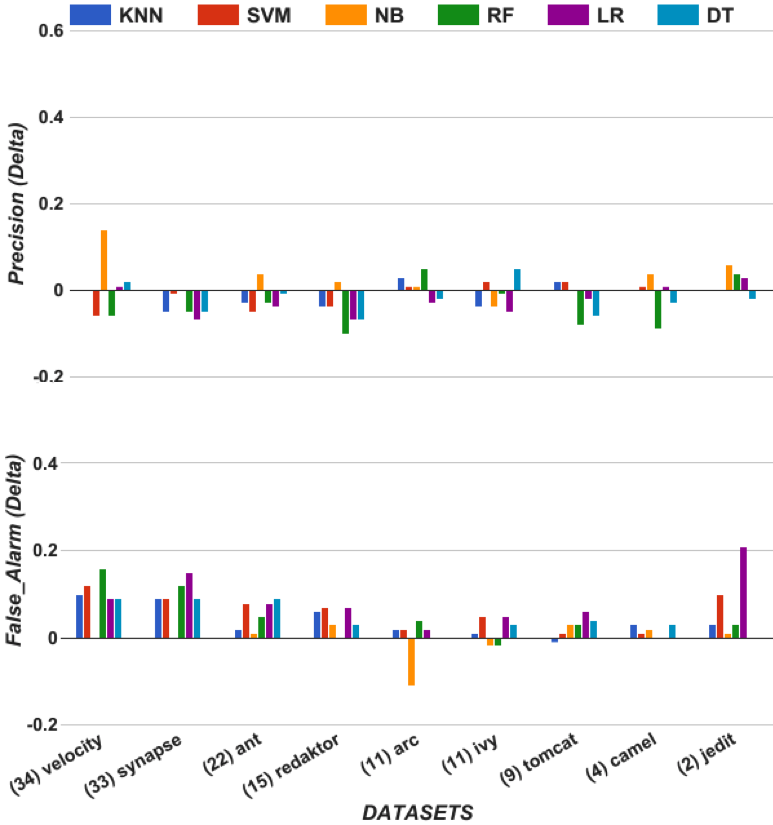
\includegraphics[width=.95\linewidth]{./fig/prec_pf_tuned.png}
    \end{minipage}%
    
    \caption{SMOTE2 improvement over SMOTE1. Legends represent the classifiers mentioned in \tion{classes}.}
    \vspace{-10pt}
    \fnote{For subfigures (AUC, Recall and Precision): larger y-values are {\em better}, if the y-value goes {\em negative}, then the corresponding learner trained on SMOTE2 data performs {\em worse} than learner learnt on SMOTE1 data. For false alarms, the plot must be interpreted differently: larger y-values are {\em worse}, if the y-value goes {\em positive}, then the corresponding learner trained on SMOTE2 data performs {\em worse} than learner learnt on SMOTE1 data. The corresponding percentage of minority class (in this case, defective class) is written beside each dataset.}
    \label{fig:tuned}
\vspace{-0.7cm}

\end{figure*}

\section{Results}
\label{sect:results}

\subsection{\textbf{RQ1: Is standard ``off-the-shelf'' SMOTE1 preprocessing method useful for defect prediction?}}
Figure~\ref{fig:untuned} represents the improvement of SMOTE1 (median value) against the No-SMOTE (median value) results and Figure~\ref{fig:tuned} represents the improvement of SMOTE2 (median value) against SMOTE1 (median value) results. Each figure contains subfigures for all our 4 evaluation measures (mentioned in \tion{measure}) compared with 6 learners (mentioned in \tion{classes}). 



For subfigures (AUC, Recall and Precision) in each Figure~\ref{fig:untuned} and \ref{fig:tuned}:
\bi
\item 
{\em Larger} y-values
are {\em better} 
\item
If the y-value goes {\em negative}, then the corresponding learner trained on SMOTE1/SMOTE2 data is {\em worse} than learner learnt on raw/SMOTE1 data respectively. 
\ei
For the false alarms, the
plots must be interpreted differently:
\bi
\item
{\em Larger} y-values are {\em worse};
\item
If the y-value goes {\em positive} then the corresponding learner trained on SMOTE1/SMOTE2 data is {\em worse} than learner learnt on raw/SMOTE1 data respectively.
\ei
In both the figures, the
X-axis shows all 9 datasets in the decreasing percentage of defective classes from left to right. The corresponding percentage of minority class (defective class) is written beside each dataset. 
According to the proponents
of SMOTE, SMOTE's improvements should
{\em increase} as we move left to right
across those plots.

For many of the results in  Figure~\ref{fig:untuned}, the changes
resulting from applying SMOTE1 are very modest. (often, less than 20\%).
The two consistent exceptions to that pattern are:
\bi
\item 
KNN seems to be effected by SMOTE1 more than any other learner.
\item 
Occasionally, SMOTE1 leads to dramatic drops in precision but in many cases, they are not statistically significant different as show in Figure~\ref{fig:stats}.
\item 
Looking left-to-right across
Figure~\ref{fig:untuned}c, we see more
large positive increases on the
right-hand-side than the left.   
\ei

We are not seeing improvement in precision is because of the way in which SMOTE works. False positives (from Figure~\ref{fig:cmatrix}) do not get reduced after applying SMOTE. SMOTE generates synthetic examples within defective data samples and its neighbors making more denser region for positive samples. So if there are any actual negative samples surrounding these denser regions will now get wrongly classified as positive by learners. 

% Based on these results,  we can best recommend SMOTE1 when:
% \bi
% \item Trying to improve recall
% for imbalanaced datasets;
% \item
% Using NB or Random Forests.
% \ei

% For SMOTE2 improvement over SMOTE1 (figure~\ref{fig:tuned}), AUC values are shown in subfigure~\ref{fig:tuned}a. Redaktor dataset is selected from X-axis, and yellow bar represents NB which corresponds to about $-0.08$ AUC value. This denotes that NB performed worse by tuning the parameters of SMOTE1. The original parameter settings of SMOTE1 worked the best. On the other hand for the same dataset, KNN (which is represented in dark blue bar) shows the AUC value of $0.35$. This shows KNN outperformed the ``off-the-shelf'' SMOTE1 when tuned using DE.



% By looking at the results of AUC from figure~\ref{fig:untuned}a, only 4 bars are negative, and rest all the remaining 50 bars (in total 9 datasets with 6 learners in each) have  positive effect by using SMOTE1 as a preprocessing method. We are seeing a maximum improvement of about 30\%. These improvements are quite modest as to ignore the importance of SMOTE.

% Results for precision (in figure~\ref{fig:untuned}b), are not much interesting, but the decrease in precision value is not that arduous except for the redaktor dataset. Though we will not recommend using SMOTE whenever we want higher precision value. Since precision is decreased using SMOTE, it was expected to have increased false alarm \cite{menzies2007problems} and the same is observed from figure~\ref{fig:untuned}d. There is an increase in error among false positives but the increase is very minimal.

% As for recall (figure~\ref{fig:untuned}c), only 4 bars are negative, and rest all the remaining 50 bars (in total 9 datasets with 6 learners in each) have positive effect by using SMOTE1. We are seeing a maximum improvement of about 60\%. These improvements are quite steep as to ignore the importance of SMOTE at any point for any learner. It is also observed that performance keeps increasing as target class becomes more minor and minor. This is what was expected after applying SMOTE to imbalance datasets.

\noindent
Summarizing the above:
\begin{lesson1}
We recommend SMOTE1 for improving recall, but SMOTE1 can,
sometimes, adversely affect
precision.
\end{lesson1}

\subsection{\textbf{RQ2: Can SMOTE2 achieve better results?}}

Figure~\ref{fig:tuned} shows the results
after applying SMOTE2. All these
plots show the {\em delta} between
the results obtained by SMOTE1 and SMOTE2.
Similar to Figure~\ref{fig:untuned} before, {\em positive}  values
are better for AUC, recall and precision
wile {\em negative} values are better for false alarms.

The benefit of SMOTE2's tunings is clearly evident in the AUC results of  Figure~\ref{fig:tuned}a:
all learners show large performance improvements. And from the Scott-Knott test shown in Figure~\ref{fig:stats}, SMOTE2 always have significantly best results for AUC. For recall, in most learners either SMOTE1 or SMOTE2 are significantly the same, or SMOTE2 performed better. 
Better yet,  as
shown in
Figure~\ref{fig:stats}, for precision and false alarm, SMOTE2 does
not adversely effect false alarm and precision as most of the times No-SMOTE, SMOTE1, and SMOTE2 are significantly the same.


At first glance, SMOTE2's effects on recall seem strange since they are
{\em better} for the more balanced left-hand-side datasets of
Figure~\ref{fig:tuned}c.  But recall from the above that SMOTE1 had less
of an effect on those left-hand-side datasets. That is, what we are seeing
here is that:
\bi
\item
SMOTE2 works often as well as SMOTE1 for imbalanced datasets;
\item
SMOTE2 offers additional benefits for datasets that are not greatly
imbalanced.
\ei

 



% results are dramat
% Now when we look at the results of AUC from figure~\ref{fig:tuned}a, only 1 bar is negative, and rest all the remaining 53 bars (in total 9 datasets with 6 learners in each) have  positive effect after when we tune the parameters of SMOTE1. We are seeing a maximum improvement of about 70\% and on an average 50\% for each learner in all datasets. These improvements are quite steep in nature and just to remind you that these results are improvement over SMOTE1. If we combine the results, then we can surely say to tune the parameters of SMOTE1 and train using any learner, we will get atleast 100\% improvement in most cases.

% We are seeing the similar trend of results for precision (in figure~\ref{fig:tuned}b), just like in Figure~\ref{fig:untuned}b, that even after tuning for precision, we are not seeing much improvement. Though we definitely improved precision slightly than SMOTE1 but the increment is not that large to recommend SMOTE2 or SMOTE1. And even after trying to minimise the false alarm (figure~\ref{fig:tuned}d) value, DE could not find a good parameter setting.

% As for recall (figure~\ref{fig:untuned}c), only 5 bars are negative, and rest all the remaining 49 bars (in total 9 datasets with 6 learners in each) have either positive effect or no effect after tuning. We are seeing a maximum improvement of about 65\% but the average improvement is close to 15\% for each classifiers in all datasets. But these improvements combined with SMOTE1 suggest that we should always tune SMOTE1 whenever the goal is to achieve higher recall.
In summary:

\begin{lesson1}
    For defect data, SMOTE2  
 offers   some  improvements over SMOTE1 for recall
 and dramatic improvements for AUC (pf, recall).
 The effects on precision and false alarm are similar to SMOTE1.
\end{lesson1}

%Based on these results, we strongly recommend SMOTE2 for handling not just unbalanced datasets but, in fact, for all datasets.

\begin{figure*}[!t]
    \centering
    \begin{minipage}{.33\textwidth}
    \centering
        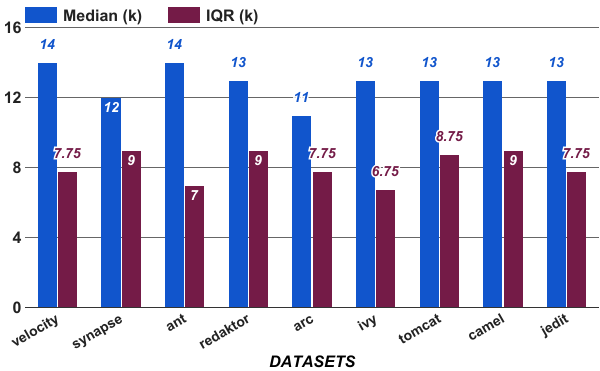
\includegraphics[width=.95\linewidth]{./fig/k.png}
        {\bf Figure~\ref{fig:para}a:} Tuned values for $k$.
    \end{minipage}%
    \begin{minipage}{.33\textwidth}
    \centering
        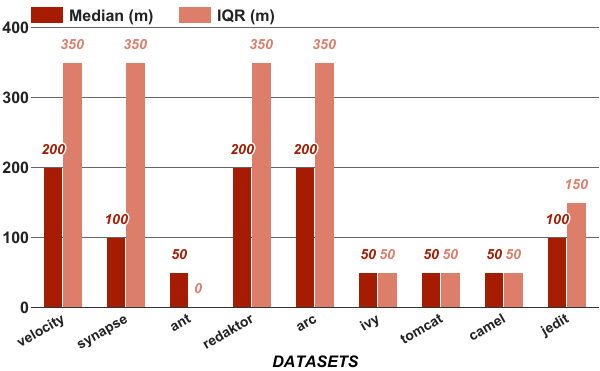
\includegraphics[width=.95\linewidth]{./fig/m.png}
        {\bf Figure~\ref{fig:para}b:} Tuned values for $m$.
    \end{minipage}
    \begin{minipage}{.33\textwidth}
    \centering
        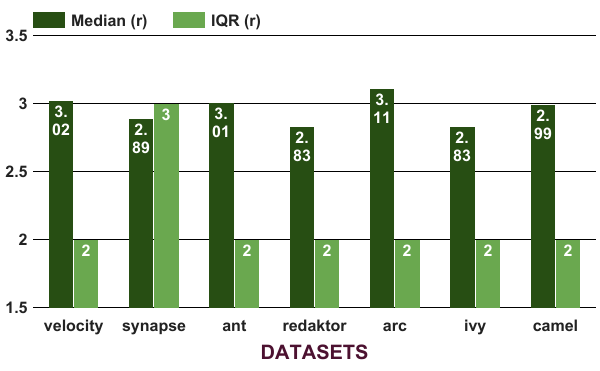
\includegraphics[width=.95\linewidth]{./fig/r.png}
        {\bf Figure~\ref{fig:para}c:} Tuned values for $r$.
    \end{minipage}
    \caption{Datasets vs Parameter Variation}
    \label{fig:para}
\vspace{-0.4cm}
\end{figure*}


\subsection{\textbf{RQ3: Does hyperparameter optimization lead to different optimal configurations for different datasets?}}

Figure \ref{fig:para} represents the parameter variations when we tuned to maximize the recall. These parameter settings are found by each learner for that dataset.
On display in each set of vertical bars are
the median values generated across 25 evaluations.
Also, shown are
the inter-quartile range (IQR) of those tunings (the IQR is the 75th-25th percentile values and is a non-parametric measure of variation
around the median value). Note that in Figure \ref{fig:para}b, IQR=0 for  ant dataset where tuning always converged on the same final value. That shows that the maximum score of recall is reached when $m=50$. No other parameter setting found out to be useful by DE.

  These figures
show how tuning selects the different ranges  of
parameters.
Some of the above numbers are far from the standard values; e.g. Chawla et al.~\cite{chawla2002smote} recommend using $k=5$ neighbors yet in our datasets, best results were seen using $k \approx 13$. On other hand it was suggested to use $m=900$ by ~\cite{pears2014synthetic}.
Clearly,
best results from tuning
vary with each dataset.

Clearly:
\begin{lesson1}
    Yes. DE finds different ``best'' parameter settings for SMOTE2 on different datasets.
\end{lesson1}
 That is,  reusing tunings  suggested  by  any other  previous study  for any dataset is \underline{{\em not}} recommended. Instead,  it is better to
      use  automatic  tuning  methods  to find the best tuning parameters for the current dataset.
      
\begin{figure*}[!t]
\begin{minipage}{.5\linewidth}
\centering
        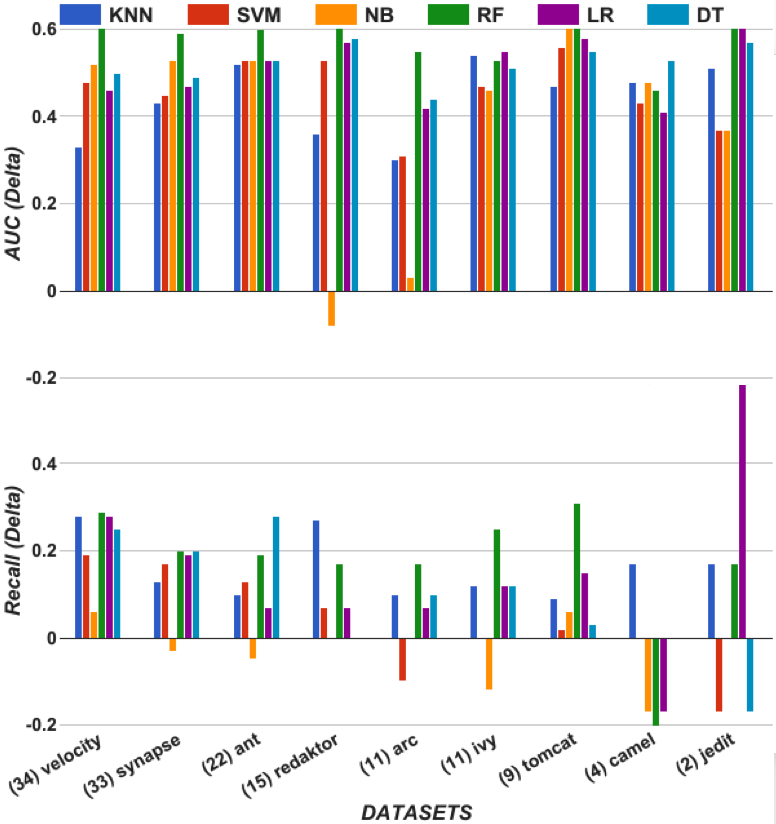
\includegraphics[width=.95\linewidth]{./fig/AUC_auc1.png}
    \end{minipage}%
\begin{minipage}{.5\linewidth}
        \centering
        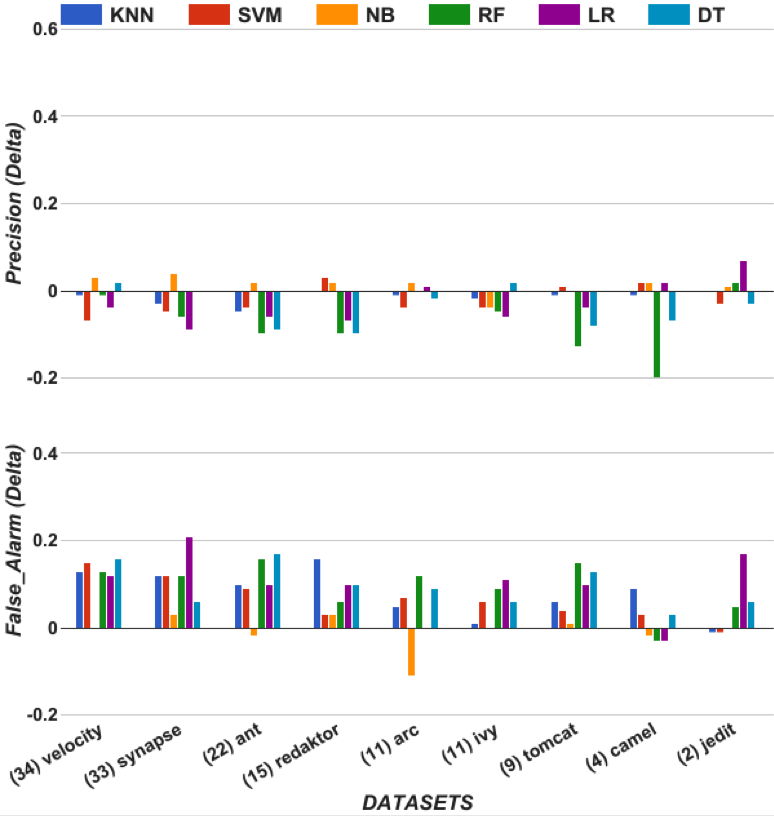
\includegraphics[width=.95\linewidth]{./fig/AUC_prec.png}
    \end{minipage}%
    
    \caption{SMOTE2 improvement over SMOTE1 when tuning goal is to maximize AUC.}
    \vspace{-10pt}
    \fnote{For subfigures (AUC, Recall and Precision): larger y-values are {\em better}, if the y-value goes {\em negative}, then the corresponding learner trained on SMOTE2 data performs {\em worse} than learner learnt on SMOTE1 data. For false alarms, the plot must be interpreted differently: larger y-values are {\em worse}, if the y-value goes {\em positive}, then the corresponding learner trained on SMOTE2 data performs {\em worse} than learner learnt on SMOTE1 data. The corresponding percentage of minority class (in this case, defective class) is written beside each dataset.}
    \label{fig:auc}
\vspace{-0.6cm}

\end{figure*} 

\subsection{\textbf{RQ4: Is tuning impractically slow?}}

Search-based SE methods can be very slow. Wang et al.~\cite{wang2013searching} once needed 15
years of CPU time to find and verify the tunings required for software
clone detectors. Sayyad et al.~\cite{sayyad2013scalable} routinely used
$10^6$ evaluations (or more) of their models in order to extract
products from highly constrained product
lines. Hence, before recommending any
search-based method, it is wise to consider the runtime cost of that
recommendation.


 Figure~\ref{runtime} shows,  in circle and square markers, the
  runtimes required to run SMOTE1 and SMOTE2 respectively.  The
  longer runtimes (in square) include the times required for DE to find
  the tunings. There is a disadvantage with SMOTE2. Figure~\ref{runtime} shows SMOTE1 reporting all the measures in the shown time. On the other hand, here SMOTE2 reports runtimes when trying to maximize recall. If it has to provide all the other 3 measures as well, it would take 3 times more than the above number which is not recommended in a real world scenario. 
  
  \begin{figure}[!htbp]
  \captionsetup{justification=centering}
  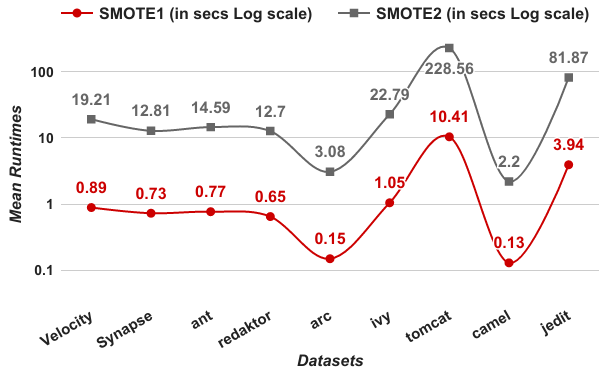
\includegraphics[width=\linewidth]{./fig/runtimes.png}
  \caption{Datasets vs Runtimes}
  \label{runtime}
\vspace{-0.7cm}
\end{figure}
  
  The work around would be is to try maximizing SMOTE2 for AUC tuning goal. AUC represents the area under the curve for pf (false alarm) and recall. When AUC improves, the heuristic is that false alarm must be getting lower and recall must be improving. And if false alarm is getting lower then precision is improving as well~\cite{menzies2007data}. We report results of AUC, Precision, Recall and False alarm in Figure~\ref{fig:auc} when we tried maximizing only AUC. We are seeing a similar conclusions as answered in our RQ2. 
  
  This additional result shows that, tuning slows down the training by a factor of up to
  five for 1 goal (which is very close to our theoretical prediction) but the improvements achieved are quite advantageous.

\begin{lesson1}
    Tuning with DE makes training four to five times slower, but the improvements in performance with respect to AUC and recall justifies the extra time required for training.
\end{lesson1}
